\documentclass[conference]{IEEEtran}
\usepackage{amsmath,amssymb,graphicx,booktabs,cite,url,iftex,balance}
\ifXeTeX
\usepackage{fontspec}
\setmainfont{texgyretermes-regular.otf}[BoldFont=texgyretermes-bold.otf,ItalicFont=texgyretermes-italic.otf,BoldItalicFont=texgyretermes-bolditalic.otf]
\fi
\newcommand{\clip}{\operatorname{clip}}
\renewcommand{\dbltopfraction}{0.85}
\renewcommand{\textfraction}{0.10}
\begin{document}
\bstctlcite{BSTcontrol}
\title{LEG-SEIR: Lagged Exposure for Graph-Based Dengue Forecasting}
\author{\IEEEauthorblockN{Anonymous Authors}}
\maketitle
\begin{abstract}
Recent local case counts provide a strong baseline for dengue forecasting, while useful cross-district signals may arrive with a delay. We propose LEG-SEIR, a compact lagged-exposure graph--SEIR forecaster. A learned sparse graph and recipient-specific lag weights jointly inform a local-preserving neural branch and imported pressure in a conservative SEIR-inspired decoder. A historical-to-simulated pressure transition connects observed reports to compartment rollout, and horizon-specific mixing combines persistence, local, graph and mechanistic forecasts. We evaluate the model using source-audited Sri Lankan district reports, development-only learning-rate selection and five-seed retrospective testing on 2026 observations. LEG-SEIR achieves mean count RMSE of 79.63, compared with 87.38 for persistence, 81.39 for an identity MLP and 80.76 for a competitive shared-adapter control. Removing the graph or replacing the mechanistic branch increases mean RMSE to 84.16 and 81.26. The improvement is strongest beyond the first horizon. These findings support the complete architecture on this sample, but do not isolate each coupling mechanism or establish prospective generalization. Frozen notebooks, source ledgers, predictions and checkpoints support independent verification.
\end{abstract}
\begin{IEEEkeywords}
dengue forecasting, graph neural networks, lagged exposure, SEIR, reproducibility
\end{IEEEkeywords}

\section{Introduction}
Dengue forecasts should be evaluated against simple surveillance-based alternatives~\cite{johansson2016evaluation,johansson2019challenge}. Sri Lanka has experienced substantial dengue outbreaks~\cite{tissera2020severe}, and forecasting challenges emphasize comparable evaluation of epidemic predictions~\cite{johansson2019challenge}. At district level, a simple forecast repeats the latest reported count. This persistence baseline requires no training. In our matched evaluation, it achieves RMSE 87.38; several simple controls improve on it (Table~\ref{tab:main}). The research question is whether a coupled spatial--mechanistic model can improve further without losing those competitive local predictors.

Lagged neighbourhood signals have motivated spatial epidemic forecasting~\cite{liucao2026,epignn2022}. We hypothesize that preserving a local predictor while selectively incorporating historical spatial information can improve this task. A compartment decoder also requires an explicit rule for transitioning from observed history to simulated states. These are design motivations tested through forecasting comparisons, rather than established transmission mechanisms.

We investigate this design question through \emph{Lagged-Exposure Graph--SEIR} (LEG-SEIR). A compact shared multilayer perceptron (MLP) models local histories. A learned directed graph and recipient-specific lag weights reuse historical information in two paths: neural graph messages and imported pressure inside an SEIR-inspired rollout. A decaying historical anchor transitions to pressure from simulated neighbour states. A learned horizon-specific mixture retains persistence alongside local, graph and mechanistic outputs.

The complete architecture achieves lower retrospective 2026 count RMSE than persistence, identity MLP and a competitive shared-adapter baseline. The latter comparison is modest, and the identity MLP remains competitive in development. The case study contains only 18 eligible origins and had previously influenced architecture ideas; it is not an untouched prospective test.

Our contributions are: (1) a compact lagged-exposure coupling that connects a local-preserving graph encoder to an imported-pressure compartment rollout; (2) a multi-fold development and matched-control evaluation, retaining simple neural baselines and negative evidence; and (3) a source-audited, independently verified experiment package. We claim a proposed design and observed improvement, not the first graph--compartment forecaster or identified biological transmission.

\section{Related Work}
\textbf{Spatial and local predictors.} Graph WaveNet and MTGNN learn spatial dependencies~\cite{wu2019graphwavenet,mtgnn2020}. Our static sparse receiver/sender graph follows this broad adaptive-graph approach. STID demonstrates strong MLP forecasting with spatial/temporal identity~\cite{stid2022}, while simple linear models can rival complex time-series architectures~\cite{zeng2023nlinear}. These findings motivate local controls; their original tasks are not dengue comparisons.

\textbf{Hybrid epidemic models.} IeRNN combines epidemic recursion and neural neighbouring effects~\cite{iernn2020}; CausalGNN couples graph learning with epidemic equations~\cite{causalgnn2022}. STAN and MPSTAN incorporate transmission-domain knowledge~\cite{stan2020,mpstan2023}. MepoGNN shares a learned graph across neural and metapopulation modules and weights mobility history~\cite{mepognn2023}. HeatGNN models mechanistic heterogeneity~\cite{heatgnn2024}, and M-Graphormer combines spatiotemporal learning with infectious-disease dynamics~\cite{mgraphormer2025}. Thus neither graph--compartment coupling nor historical weighting alone is new.

\textbf{Dengue and lagged influence.} Liu and Cao include lagged neighbourhood memory in multi-disease forecasting~\cite{liucao2026}. Weng et al. study Sri Lankan dengue graph forecasting with environmental inputs~\cite{weng2024graph}; Liu et al. develop an explainable covariate compartmental model for Sri Lankan dengue~\cite{liu2025seirlstm}. Their tasks and inputs differ from our case-only comparison. Our proposed contribution is the specified reuse of recipient-specific case-lag weights in neural messages and imported pressure, with a historical-to-simulated pressure transition and horizon mixing. Published mechanisms above are context, not reproduced competitors in our final table.

\textbf{Anchoring and evaluation.} Persistence initialization has been studied in neural forecasting~\cite{haugsdal2023persistence}. We retain persistence as a jointly trained mixture component. Forecasting evaluations require comparable targets~\cite{johansson2016evaluation,johansson2019challenge}; repeated selection can overfit finite validation data~\cite{cawley2010selection}. We select learning rates on pre-2026 folds and explicitly describe the previously inspected case study as retrospective.

\section{The LEG-SEIR Forecaster}
\subsection{Task and overall computation}
At origin $t$, input $C_t\in\mathbb R^{N\times L}$ contains $L$ observed reports for $N$ districts, ending at $t-1$. We predict the next $H$ reports, $Y_t\in\mathbb R^{N\times H}$. Columns $\ell=1,\ldots,L$ run from oldest to latest. Figure~\ref{fig:architecture} shows the main dependencies. Raw counts initialize the decoder, while standardized logs supply the neural branches. A local representation is retained through a gated residual graph message. All four outputs are mixed before transformation back to counts.

\begin{figure*}[t]
\centering
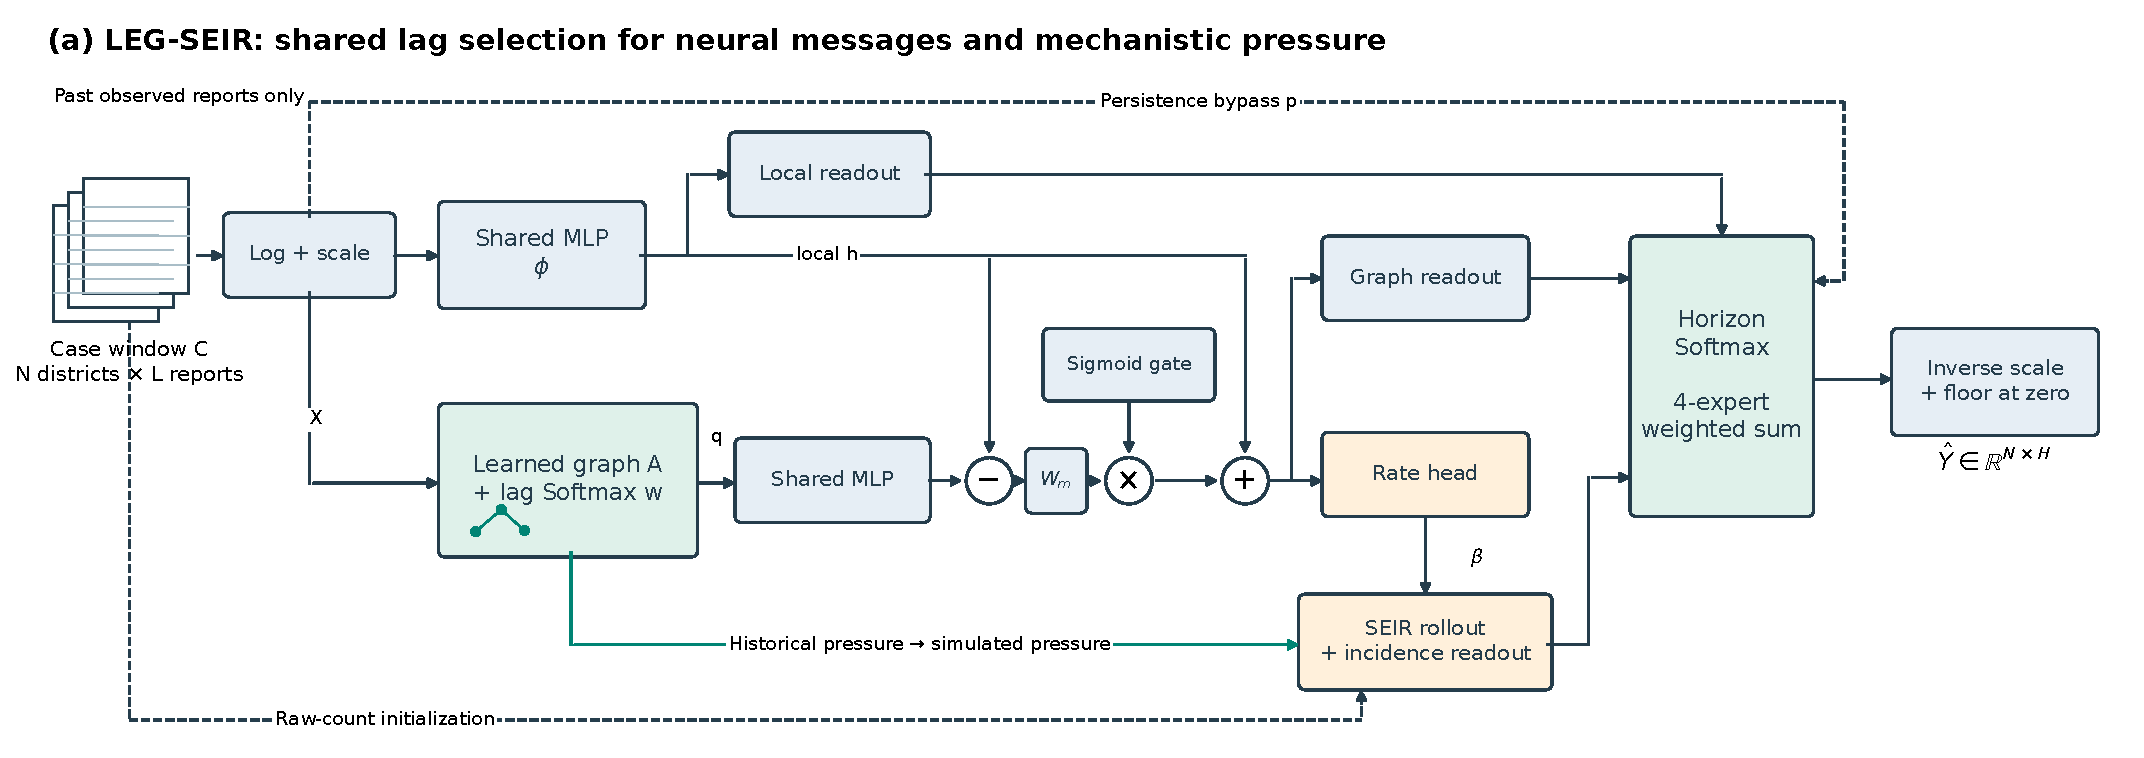
\includegraphics[width=\textwidth]{figures/architecture.pdf}
\caption{LEG-SEIR architecture. Standard MLP/readout blocks are kept compact; green components highlight the proposed lag coupling and prediction fusion. The same graph and lag weights feed neural history aggregation and mechanistic imported pressure. Subtraction, linear projection, gating and addition preserve a local representation. Dashed paths carry raw counts and the persistence bypass. The local and graph readouts share parameters. Learned connections are predictive dependencies, not measured transmission routes.}
\label{fig:architecture}
\end{figure*}

Let $X=(\log(1+C)-\mu)/\sigma$, using training-only scalar statistics, and $p_{i,h}=X_{i,L}$ repeat the latest observation. The shared encoder $\phi$ reads levels and their consecutive differences:
\begin{equation}
h_i=\phi(X_i,\Delta X_i),\qquad f^L_i=W_o h_i+b_o.
\end{equation}
The evaluated encoder has no district-ID input embedding. District-specific graph factors and lag parameters still condition the model; it is not an unseen-district inductive architecture.

\subsection{Shared graph and historical lag selection}
Learned receiver/sender factors $U,V\in\mathbb R^{N\times d_a}$ give scores $UV^\top$. Mask the diagonal, retain the largest $K_g$ off-diagonal entries per receiver, and apply row-softmax to obtain $A$. Thus $A_{ij}$ weights sender $j$ for receiver $i$. The graph is learned during training and fixed during inference, rather than an input-dependent attention matrix.

Each receiving district has lag logits $\ell_i\in\mathbb R^L$, with $w_i=\operatorname{softmax}(\ell_i)$. The factorized operator $A_{ij}w_{i,l}$ separates spatial weighting from historical selection. The lag-weighted neural input and representation are
\begin{align}
q_{i,l}&=Lw_{i,l}\sum_j A_{ij}X_{j,l},\label{eq:lag}\\
h_i^G&=h_i+g_G W_m[\phi(q_i,\Delta q_i)-h_i],\quad
g_G=\operatorname{sigmoid}(a_G).\label{eq:message}
\end{align}
The factor $L$ makes uniform lag weights recover the ordinary graph-averaged history. The same encoder processes $q$, including its differences. Subtracting $h_i$ forms a neighbour departure; gated addition retains the local path. The graph forecast reuses the local head: $f_i^G=W_o h_i^G+b_o$. Lag weights are recipient-specific, shared across senders and origins; they are not edge-specific incubation or travel delays.

\subsection{Imported pressure and observation-to-simulation bridge}
For fixed population $P_i$, let $K_i=P_i/11$ and $c^*_{i,l}=\clip(C_{i,l}/K_i,10^{-6},0.5)$. The same graph and lag weights construct a historical imported-pressure anchor:
\begin{equation}
a_i=\sum_l w_{i,l}\sum_j A_{ij}c^*_{j,l}.
\end{equation}
A rate head maps $h_i^G$ to $H$ logits $r_{i,h}$, converted to positive transmission proxies $\beta_{i,h}$. During solver day $k$, all districts have simulated infectious fractions $i_j(k)$. Historical pressure gradually gives way to these states:
\begin{align}
n_i(k)&=\sum_j A_{ij}i_j(k),\quad d_k=\exp(-k/\tau),\\
P_i(k)&=d_k a_i+(1-d_k)n_i(k),\label{eq:bridge}\\
\lambda_i(k)&=\beta_{i,h}[(1-\eta)i_i(k)+\eta P_i(k)],
\quad\eta=\operatorname{sigmoid}(a_\eta).\label{eq:force}
\end{align}
Figure~\ref{fig:bridge} separates the historical-to-simulated transition from local/import gating. At $k=0$, imported pressure uses the observed anchor; later steps increasingly use simulated neighbours. The decay constant is fixed. There is no assimilation of future reports during rollout.

\begin{figure*}[t]
\centering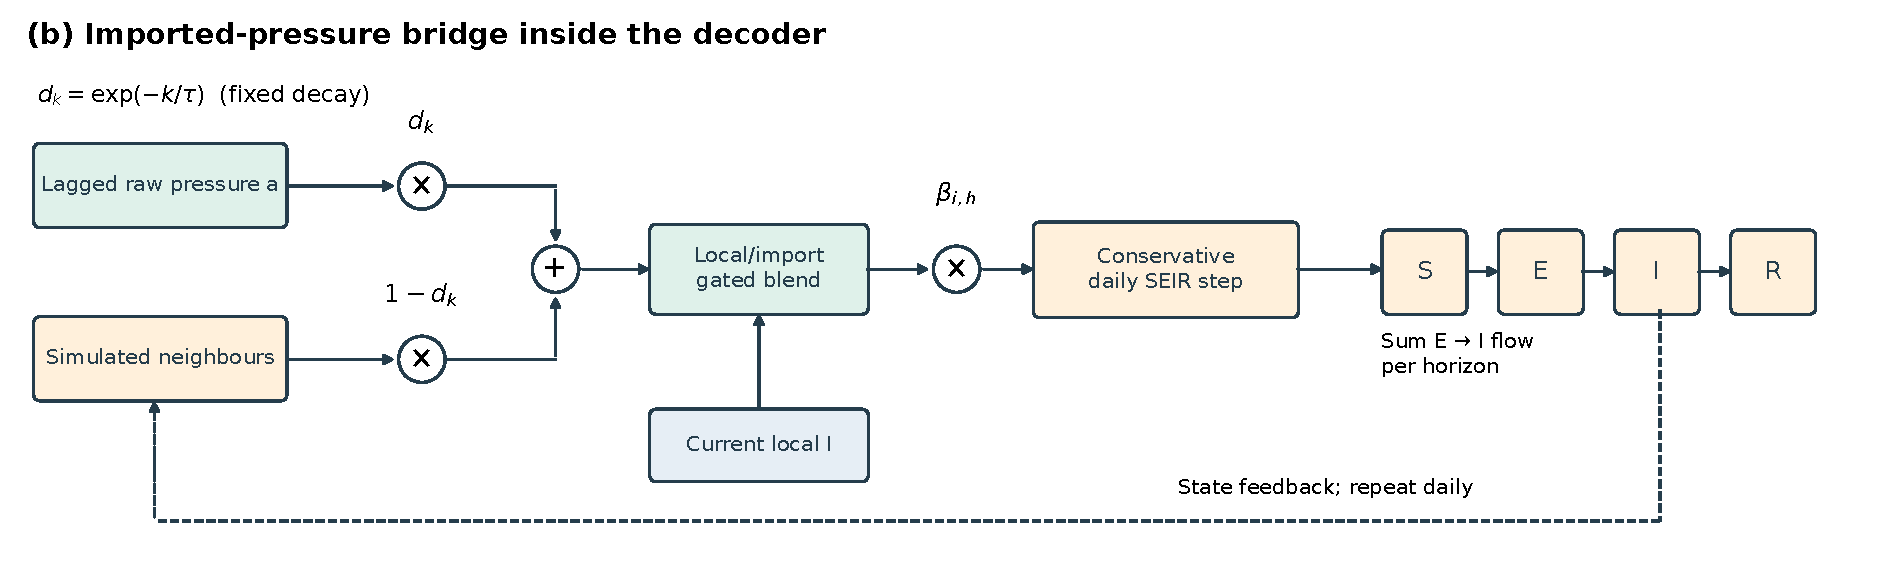
\includegraphics[width=\textwidth]{figures/pressure_bridge.pdf}
\caption{Imported-pressure bridge. Historical and simulated neighbour pressure are weighted by $d_k$ and $1-d_k$, summed, then blended with local infectious pressure through a shared learned gate. The neural rate supplies infection force to a conservative SEIR-inspired step. Simulated infectious states feed the next daily step; exposed-to-infectious flows provide the incidence-style readout. This schematic describes computation, not validated disease mechanisms.}
\label{fig:bridge}
\end{figure*}

\subsection{Conservative incidence decoder}
SEIR partitions a population into susceptible, exposed, infectious and removed states~\cite{gopalakrishnan2020seir}. Here normalized fractions are \emph{proxies}. At each origin, initialize $s=0.318$, $e=c^*_{i,L-1}$, $i=c^*_{i,L}$, and $r=\max(0,1-s-e-i)$, then normalize to unit mass. Each daily step computes bounded pre-update flows:
\begin{align}
u&=s(1-e^{-\lambda}),\quad v=e(1-e^{-\omega}),\nonumber\\
z&=i(1-e^{-\gamma}),\\
s^+&=s-u,\quad e^+=e+u-v,\nonumber\\
i^+&=i+v-z,\quad r^+=r+z.
\end{align}
Every outflow is bounded by its source compartment, preserving nonnegativity and total mass. Sum $v$ over $D$ daily steps per horizon and scale by $K_i$ to produce $y^S_{i,h}$. Transform this output to standardized log space $f^S$. Numerical conservation does not validate biological states, and the decoder does not explicitly represent mosquitoes, serotypes or reinfection. Vector--host SEIR--SEI models explicitly represent mosquito compartments~\cite{seirsei2022,phaijoo2018sensitivity}.

\subsection{Horizon mixing and learning objective}
Learned horizon logits $\theta\in\mathbb R^{H\times4}$ yield four softmax weights, shared across districts and origins:
\begin{equation}
\widehat z_{i,h}=\alpha_{h,p}p_i+\alpha_{h,L}f^L_{i,h}
+\alpha_{h,G}f^G_{i,h}+\alpha_{h,S}f^S_{i,h}.
\end{equation}
Inverse transformation gives $\widehat y=\max(0,\exp(\mu+\sigma\widehat z)-1)$. Mixing occurs in log space, not count space. The head learns a separate four-expert mixture for each horizon. Experts learn jointly, so mixture weights do not identify causal contributions or the quality of separately trained predictors.

For training origins $\mathcal T$, the objective is
\begin{equation}
\mathcal L=\frac{1}{|\mathcal T|NH}\sum_{t\in\mathcal T,i,h}
(\widehat z_{t,i,h}-z_{t,i,h})^2.
\end{equation}
Checkpoint selection instead minimizes validation count RMSE; the two criteria emphasize different errors.

\section{Data and Experimental Protocol}
\subsection{Source reconstruction and eligible windows}
We reconstruct counts from Sri Lanka's Epidemiology Unit Weekly Epidemiological Reports\footnote{\url{https://www.epid.gov.lk/weekly-epidemiological-report/weekly-epidemiological-report}} and use Census 2012 population tables\footnote{\url{https://www.statistics.gov.lk/}}. The curated source snapshot is pinned by its manifest. The source manifest contains 714 entries, including 685 original report PDFs across 686 report slots through Vol.~53 No.~33. Aggregating Ampara and Kalmunai maps 26 reporting divisions to 25 districts. Only case histories and fixed population scaling enter the model; no mobility, boundaries or weather are inputs.

The frozen source policy accepts coherent printed counts and documented arithmetic repairs, retaining unresolved reports as missing. Identical coherent cumulative counts accompanying repeated positive weekly counts cannot certify zero incidence. No count is removed because of its forecast error. Incomplete input/target windows are excluded; the supplement records parsing, repairs and coverage. Code is maintained in the project repository\footnote{\url{https://github.com/rathishTharusha/leg-seir}}; the audited tables and experiment evidence are available on Hugging Face\footnote{\url{https://huggingface.co/datasets/rathishTharusha/leg-seir}}..

Targets use report-period year, not recovered release vintages. Forecast horizons are subsequent report observations, whereas the decoder assumes seven daily steps per horizon. This mismatch and retrospective source reconstruction limit operational interpretation. Final splits contain 525 training origins through 2024, 40 validation origins in 2025 and 18 test origins in 2026. All compared methods use identical eligible target windows; earlier observed 2026 reports may enter later rolling test inputs, but test targets never update parameters.

\subsection{Development selection and final fits}
A pre-2026 validation screen shortlisted three families: horizon mixture, lagged exposure and compartment-only observer. Development A trains through 2022 and validates 2023; B trains through 2024 and validates 2025. Fifteen configurations, two learning rates and three seeds in both folds give 180 fits. Each configuration selects the LR maximizing mean fold skill $1-\mathrm{RMSE}/\mathrm{RMSE}_{\rm persistence}$; ties favour the lower LR. Matched removals retain their parent's LR.

Final training through 2024 selects checkpoints on 2025 and scores 2026 using five seeds. Seventy-five primary fits and ten additional horizon-removal LR sensitivities bring the total to 265 neural fits, plus three fixed-alpha ridge fits. Selection seeds 0--2 overlap final seeds 0--4. The supplement provides the chronology and selection records. LEG-SEIR was shortlisted before final fitting, but 2026 had previously influenced research ideas; this comparison is retrospective.

\subsection{Controls and implementation}
Controls include persistence, shared ridge ($\alpha=1$; five level/difference inputs), local MLP, identity MLP, plain graph, local SEIR, uniform mixture, shared adapter, horizon mixture and compartment-only observer. The identity MLP adds a learned four-dimensional district embedding. The shared adapter uses a rank-eight correction with its adapter parameters exempted from weight decay. Complete wiring and capacities are supplied; matched training recipes do not imply identical parameter counts.

LEG-SEIR graph removal disables both neural graph messages and imported pressure; its mechanistic replacement retains lagged neural messages but replaces the SEIR output with a direct neural branch. These controls do not isolate imported pressure or the decay transition individually. Local SEIR uses the inherited two-stage anchored blend, whereas graph-off uses a four-expert mixture; they are distinct controls.

In the evaluated implementation, $N=25$, $L=H=3$, width is 64, $d_a=8$, $K_g=5$, $D=7$, $\tau=7$, $\omega=0.1$ and $\gamma=1/7$. Transmission is $\beta=\exp[\clip(r-1.1,-9,1.1)]$. Graph/import gate logits initialize at $-2$; lag and mixture logits at zero. LEG-SEIR has 9,519 parameters versus identity MLP's 5,095. Adam~\cite{kingma2015adam} uses batch 128, weight decay $10^{-4}$, gradient clipping at 5, at most 300 epochs and patience 40. LEG-SEIR's selected LR is 0.003; identity MLP and shared adapter use 0.001. Runtime versions and source hashes are in the supplement and execution archive.

\subsection{Metrics and verification}
Count RMSE pools origins, districts and horizons equally:
\begin{equation}
\mathrm{RMSE}=\sqrt{\frac{1}{ONH}\sum_{t,i,h}(\widehat y_{t,i,h}-y_{t,i,h})^2}.
\end{equation}
We report the mean and sample SD of five seed-specific RMSEs, not ensemble RMSE or a confidence interval. MAE and sMAPE are secondary; percentage measures require care near zero~\cite{hyndman2006accuracy}. With 18 overlapping origins, the 1,350 scored cells are not independent samples; dependence also matters for resampling uncertainty~\cite{kunsch1989bootstrap}. No significance claim is made. Verification checks 915 hashes, all 265 neural CPU reloads, reconstructed metrics, source truths, scaling, chronology and LR selection; it does not refit ridge.

\section{Results}
\subsection{Observed improvement and competitive controls}
Table~\ref{tab:main} and Fig.~\ref{fig:results} compare the primary sample. LEG-SEIR reaches $79.63\pm0.64$ RMSE, 8.87\% below persistence and 2.16\% below identity MLP. Shared adapter reaches $80.76\pm0.38$; LEG-SEIR's relative RMSE reduction against it is only 1.39\%. This competitive result must remain visible. LEG-SEIR also has lower mean MAE than identity MLP, but not every secondary metric favours it over every removal.

\begin{table}[t]
\centering\caption{Primary 2026 results. Neural RMSE: mean $\pm$ sample SD over five seeds; MAE: seed mean. Same 18 origins for all rows.}
\label{tab:main}\begin{tabular}{lrr}\toprule Method & RMSE & MAE\\\midrule
Persistence & 87.38 & 34.69\\
Shared ridge & 85.54 & 34.93\\
Local MLP & $84.86\pm1.39$ & 33.80\\
Identity MLP & $81.39\pm0.72$ & 32.50\\
Plain graph & $82.63\pm1.02$ & 33.23\\
Local SEIR & $84.89\pm3.17$ & 33.72\\
Uniform mixture & $83.15\pm4.17$ & 33.19\\
Shared adapter & $80.76\pm0.38$ & 32.45\\
Horizon mixture & $81.75\pm1.28$ & 32.68\\
Compartment observer & $81.76\pm1.59$ & 32.88\\
LEG-SEIR (proposed) & $79.63\pm0.64$ & 32.14\\
LEG-SEIR: neural replacement & $81.26\pm0.57$ & 32.87\\
LEG-SEIR: graph removed & $84.16\pm2.86$ & 33.52\\
\bottomrule\end{tabular}
\end{table}
\begin{figure*}[t]
\centering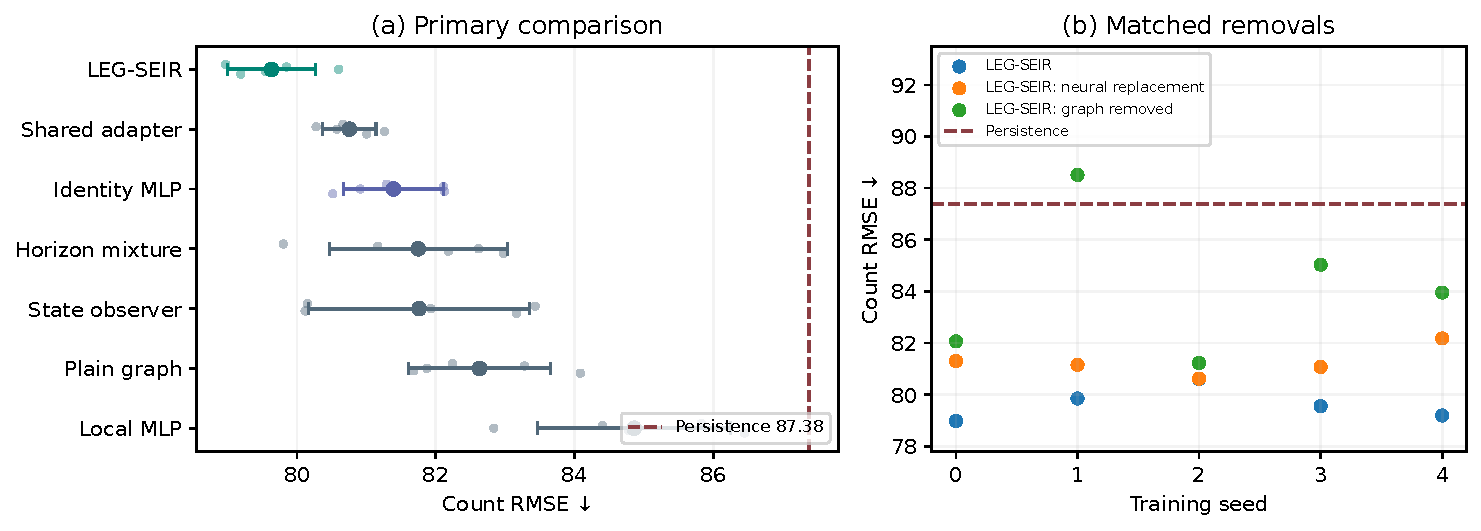
\includegraphics[width=.97\textwidth]{figures/results_comparison.pdf}
\caption{Primary comparison and matched removals. (a) Large points show mean RMSE, bars show training-seed SD and small points show individual seeds; bars are not confidence intervals. (b) The complete model beats both removal controls in each seed, but the seed-two mechanistic difference is small. Graph removal jointly changes neural messages and imported pressure.}
\label{fig:results}
\end{figure*}

\subsection{Development evidence and horizon dependence}
At the chosen rates, LEG-SEIR has mean development RMSE 50.86 in 2023 versus identity MLP's 51.17. In 2025, identity MLP slightly leads: 19.32 versus 19.34. These results constrain any general claim of graph superiority. Final horizon RMSEs for LEG-SEIR are 41.83, 80.52 and 103.87, compared with persistence at 42.63, 89.22 and 114.58 (Fig.~\ref{fig:horizons}). Most improvement occurs beyond the first horizon; not every seed improves first-horizon error.

\begin{figure*}[t]
\centering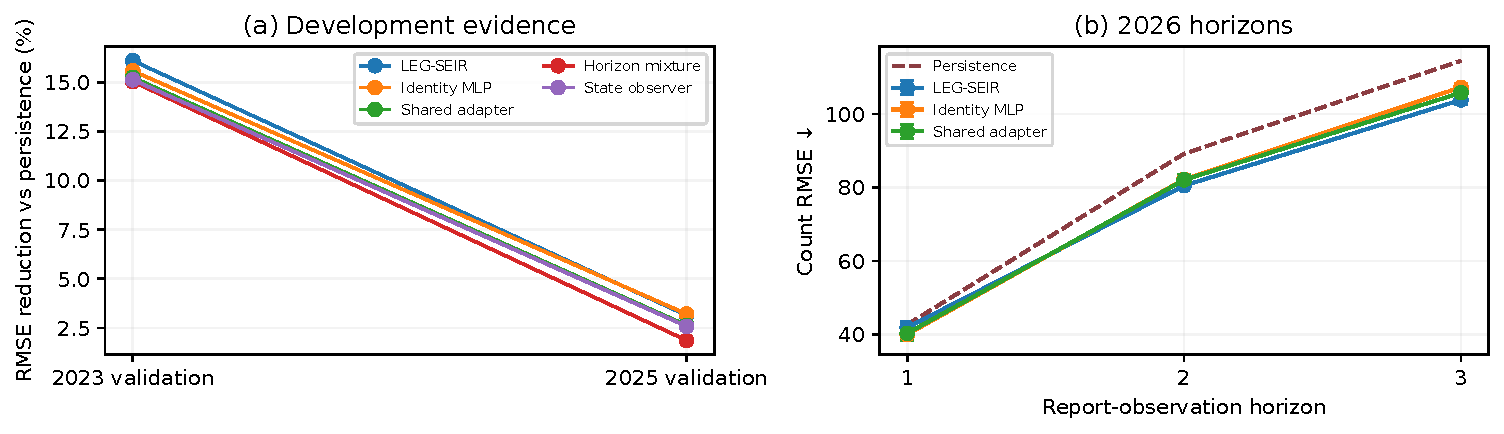
\includegraphics[width=.97\textwidth]{figures/development_horizons.pdf}
\caption{Development and horizon evidence. (a) Fold-specific skill at development-selected learning rates; identity MLP remains competitive, especially in 2025. (b) Five-seed mean count RMSE by horizon, with seed SD. The proposed model's larger gains occur at horizons two and three.}
\label{fig:horizons}
\end{figure*}

\subsection{What the component comparisons establish}
Graph removal gives 84.16 RMSE; mechanistic replacement gives 81.26. The complete model wins both comparisons in all five seeds, but the seed-two difference against replacement is approximately 0.01848 RMSE. This supports the complete configuration on these observations, not a separately established advantage for each pressure mechanism. The original no-import screen had mixed seed effects and used a smaller budget.

SEIR is not universally helpful: the ordinary horizon mixture scores 81.75, whereas its direct replacement scores 81.36 at the parent's LR. The compartment-only observer reaches 81.76. Additional horizon-removal LR sensitivities and all negative results are retained in the supplement. The final comparison evaluates three shortlisted families and controls, not all nine screened families.

Supplementary national-total curves use five-seed ensembles rather than district-pooled seed scores. They still lag some rapid growth and overpredict later observations; lower pooled RMSE does not imply accurate prediction of every outbreak phase.

\section{Discussion and Conclusion}
The evidence supports a compact coupled forecaster on this retrospective sample. The scientific motivation is to use historical spatial information without replacing the local predictor, then transition that information into simulated pressure for longer horizons. Lower error than the identity MLP and matched removals is consistent with that motivation, but it does not identify the cause of improvement. Shared graph modelling, lagged neighbourhood influence and mechanistic neural forecasts all have precedents; the proposed contribution is their specified coupling, not those ingredients individually.

Several limits remain. First, only one country and 18 overlapping final origins are scored, and 2026 motivated earlier design choices. Second, immutable report-release vintages were not recovered, so source reconstruction is retrospective. Third, the experiment did not evaluate the alternative printed-repeat reporting policy. Fourth, the SEIR constants and seven-day solver mapping are assumptions requiring sensitivity analysis; the human-only decoder omits explicit dengue vector dynamics. Fifth, graph removal does not isolate imported pressure, and externally published hybrid models have not been rerun as matched competitors.

Further work should compare uniform and learned lag weights, isolate import gating while retaining neural messages, remove the history-to-simulation transition, and test separate versus shared coupling operators. These experiments must use development-based decisions and an independent future period or dataset, rather than repeatedly optimizing the now-seen 2026 sample. Operational use would additionally require release-vintage inputs and calibrated uncertainty.

LEG-SEIR reduces mean retrospective RMSE relative to strong simple controls while preserving a compact, explicitly specified computation. Its present value is a reproducible architectural hypothesis with supporting comparisons. Independent confirmation and targeted ablations are needed before stronger mechanism or generalization claims.

\bibliographystyle{IEEEtran}
\bibliography{references}
\end{document}
